\begin{exercise}{Compétition ente précipités}{2}{PCSI}{Chimie générale, Réactions de précipitation, Solubilité}{chocron}

On étudie la compétition entre deux précipités : en présence d'ions iodure, les ions Pb$^{2+}$ donnent un précipité jaune et les ions Hg$^{2+}$ un précipité rouge-orangé. 

\begin{questions}
\questioncours  Critère de précipitation d'un solide en solution aqueuse.

\begin{EnvUplevel}
Lorsqu'on ajoute goutte à goutte une solution contenant des ions Hg$^{2+}$ dans un tube à essais contenant un précipité d'iodure de plomb, le précipité devient rouge-orangé dès les premières gouttes.
\end{EnvUplevel}

\question Que peut-on conclure de cette observation? \'Ecrire l'équation de la réaction (R) qui modélise le phénomène.

\begin{EnvUplevel}
On dispose d'une solution d'ions iodure de concentration $\mathrm{[I^-]_0} = 4\times 10^{-3}$ mol$\cdot$L$^{-1}$ et de deux béchers contenant respectivement 20 mL d'une solution de Pb$^{2+}$ d'une part et Hg$^{2+}$ d'autre part, de concentration $C_0$ = 0,1 mol$\cdot$L$^{-1}$. 
Dans chaque bécher, on ajoute une goutte de la solution d'ions iodure : on observe la formation d'un précipité rouge-orangé dans un bécher mais l'autre solution reste limpide.
\end{EnvUplevel}

\question Donner l'équation de la réaction ayant lieu. Sachant que le volume d'une goutte est de l'ordre de 0,05 mL, en déduire une borne inférieure du produit de solubilité de PbI$_2$ et une borne supérieure de celui de HgI$_2$.

\begin{EnvUplevel}
Le document ci-dessous correspond à la simulation de l'ajout d'une solution d'ions iodure à une solution équimolaire en ions Pb$^{2+}$ et Hg$^{2+}$, toutes les deux à 0,1 mol$\cdot$L$^{-1}$ :

\begin{figure}[H]
    \centering
    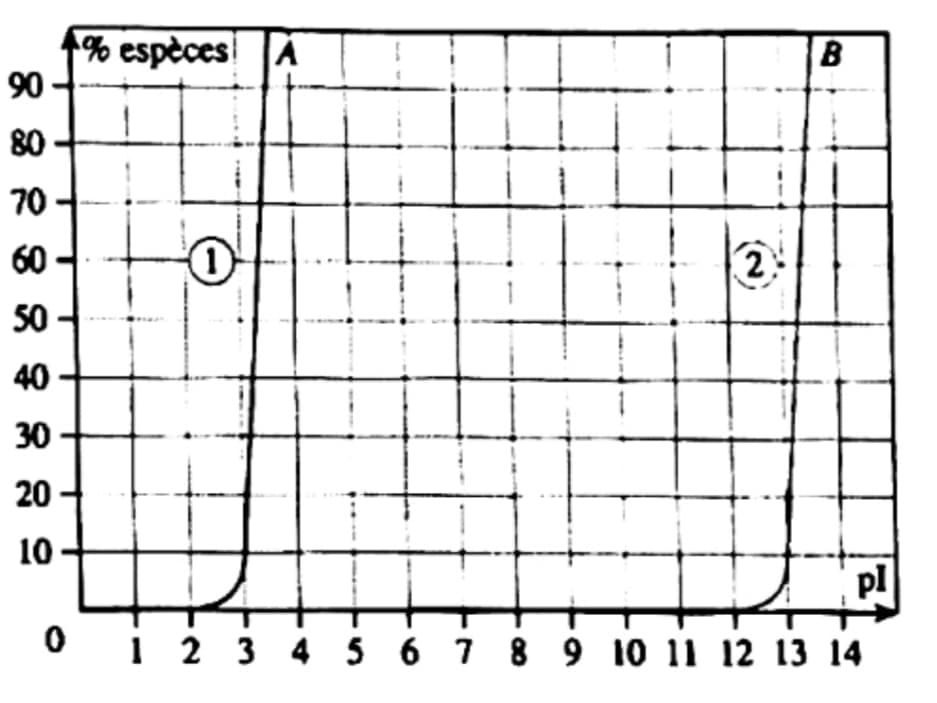
\includegraphics[width=0.8\linewidth]{chimie/precipitation/precipitationLC.jpg}
    \vspace{-1em}
    \caption[Pourcentage de cations métalliques présents dans des solutions d'ions Pb$^{2+}$ et d'ions Hg$^{2+}$  en fonction de la concentration d'ions I$^-$ ajoutés $\mathrm{pI = -\log [\text{I}^-]}$.]{Pourcentage de cations métalliques présents dans des solutions d'ions Pb$^{2+}$ et d'ions Hg$^{2+}$ en fonction de la concentration d'ions I$^-$ ajoutés $\mathrm{pI = -\log [\text{I}^-]}$.}
\end{figure}
\end{EnvUplevel}

\question Que représentent les points anguleux? Identifier les deux courbes tracées (on note que les courbes \textcircled{1} et \textcircled{2} sont strictement égales à 100\% à droite des points A et B respectivement)

\question  En déduire les produits de solubilité de PbI$_2$ et HgI$_2$. Commenter.

\question Déterminer la constante d'équilibre de la réaction (R). Commenter.

\end{questions}
\end{exercise}

\begin{solution}
\begin{questions}

\questioncours Exemple de HgI$_2$. La réaction $\mathrm{HgI_2}_\text{s} \leftrightharpoons \mathrm{Hg^{2+}_\text{aq} + 2 {I^-}_\text{aq}}$ admet pour constante d'équilibre $K_s$. Le solide n'existe que pour $Q_r > K_s$ :
    \begin{center}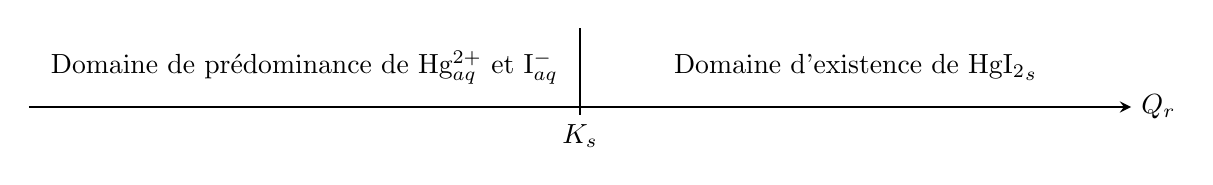
\begin{tikzpicture}[baseline=1em]
        \draw[->, >=stealth, thick] (-7,0)--(7,0) node[right]{$Q_r$};
        \draw[black] (0,1)--(0,-0.1) node[below]{$K_s$} ;
        \node at (-3.5,.5) {Domaine de prédominance de Hg$^{2+}_\text{aq}$ et I$^-_\text{aq}$};
        \node at (3.5,.5) {Domaine d'existence de $\mathrm{HgI_2}_\text{s}$};
    \end{tikzpicture}\end{center}

\question Lorsqu'on introduit des ions mercuriques dans une solution en présence de précipité d'iodure de plomb, le précipité de plomb (jaune) disparaît et le précipité de mercure (rouge-orangé) apparaît.
Il se produit donc la réaction
\begin{equation}
    \mathrm{{PbI_2}_\text{(s)} + {Hg^{2+}}_\text{(aq)} \rightleftharpoons {Pb^{2+}}_\text{(aq)} + {HgI_2}_\text{(s)}} \qqtext{de constante} K. \tag{R}
\end{equation}
    
Cette réaction est très favorable dans le sens direct ($K\gg 1$).
HgI$_2$ est donc moins soluble dans l'eau que PbI$_2$.


\question Il y a formation d'un précipité rouge-orangé donc HgI$_2$. La réaction de formation est
$$\mathrm{Hg^{2+} + 2I^- \rightarrow HgI_2}.$$

D'après le critère de précipitation en solution, le précipité se forme si $Q_r > K_{s,\mathrm{HgI_2}}$, donc $$\mathrm{[Hg^{2+}][I^-]^2}  \geqslant K_{s,\mathrm{HgI_2}}, \quad \Longleftrightarrow \quad \mathrm{[Hg^{2+}] = 0,1 \ mol\cdot L^{-1}},$$
en négligeant la variation de volume $V_g$ ajouté par la goutte.
$$\mathrm{[I^-]= [I^-]_0} \dfrac{V_g}{V_0} = \mathrm{1\cdot10^{-5} mol\cdot L^{-1}}$$

On a donc $Q_r = 10^{-11} \geqslant K_{s,\mathrm{HgI_2}},$

Avec le même calcul pour PbI$_2$, et dans ce cas, comme le précipité ne se forme pas, $Q_r \leqslant K_s$, on trouve 
10$^{-11} \leqslant K_{s,\mathrm{PbI_2}}$.

\question Initialement la solution ne contient pas de I$^-$ (pI $\rightarrow + \infty$) et les ions Pb$^{2+}$ et Hg$^{2+}$ sont tous les deux à la concentration C$_0$ = 0,100 mol$\cdot$L$^{-1}$. En pourcentage, 100\% des cations sont en solution, la solution est limpide.

Puis on ajoute des ions I$^-$, rien ne se passe jusqu'au point B (en partant de la droite i.e. en ajoutant des ions iodure) où pI$_B = 13,6$. 

Le point B est un point anguleux de la courbe \textcircled{2} ; cela traduit \textbf{une rupture d'équilibre, en l'occurrence, l'apparition d'un précipité}. D'après la question précédente, on sait que Hg$^{2+}$ est un meilleur accepteur de I$^-$ que Pb$^{2+}$ : c'est donc le précipité HgI$_2$ qui apparaît en B. Si on continue d'ajouter du I$^-$, cela entraîne la précipitation de HgI$_2$ et donc la diminution de la concentration en Hg$^{2+}$. 
\textbf{La courbe \textcircled{2} représente donc la concentration de Hg$^{2+}$, exprimée en pourcentage de C$_0$.}

Lorsque Hg$^{2+}$ a quasiment disparu, le pI diminue de nouveau puisqu'on ajoute des ions iodure en solution. 
La courbe \textcircled{1} reste à 100\% jusqu'en A, où un nouveau point anguleux survient (pI$_A$=3,6) qui traduit l'apparition du second précipité PbI$_2$. 
\textbf{La courbe \textcircled{1} représente donc la concentration de Pb$^{2+}$, exprimée en pourcentage de C$_0$.}

\question Pour trouver les produits de solubilité, on utilise les coordonnées des points anguleux.

Par exemple, pour HgI$_2$, en B, le premier grain de précipité apparaît et donc on peut utiliser le $K_s$. Par ailleurs, la proportion de Hg$^{2+}$ est encore de 100\% donc sa concentration vaut 0,100 mol$\cdot$L$^{-1}$.
On a donc
$$K_{s,\mathrm{HgI_2}} = \mathrm{[Hg^{2+}]_B \times [I^-]_B^2} = C_0 \times 10^{-2pI_B} = 6 \cdot 10^{-29}.$$  

De même,
$$K_{s,\mathrm{PbI_2}} = \mathrm{[Pb^{2+}]_A \times [I^-]_A^2} = C_0 \times 10^{-2pI_A} = 6 \cdot 10^{-9}.$$   

Ces résultats sont en accord avec les bornes inférieure et supérieure déterminées à la question 3.

\question $K = \dfrac{K_{s,\mathrm{PbI_2}}}{K_{s,\mathrm{HgI_2}}} = 10^{+20} \gg 1$ comme prévu.

\end{questions}
\end{solution}